\item[(b)]
\section*{Exercise 2 Task (b): Analyzing the Effects of Sampling on Spectrum}

\subsection*{Objective}
This task examines the implications of sampling the signal \(x(t)\) at 8 kHz, specifically how it affects the signal's spectrum.
The focus is on identifying and visualizing the spectrum of the sampled signal \(x[n]\) from \(-f_s\) to \(f_s\) and highlighting the baseband to assess aliasing.

\subsection*{Methodology}
The spectrum of \(x(t)\), defined by specified piecewise conditions for magnitude and phase, is calculated and plotted after sampling in Figure~\ref{fig:exercise2b_spectrum}.
This process involves replicating the original spectrum at intervals of the sampling frequency and examining overlaps that indicate aliasing.

\begin{figure}[h]
    \centering
    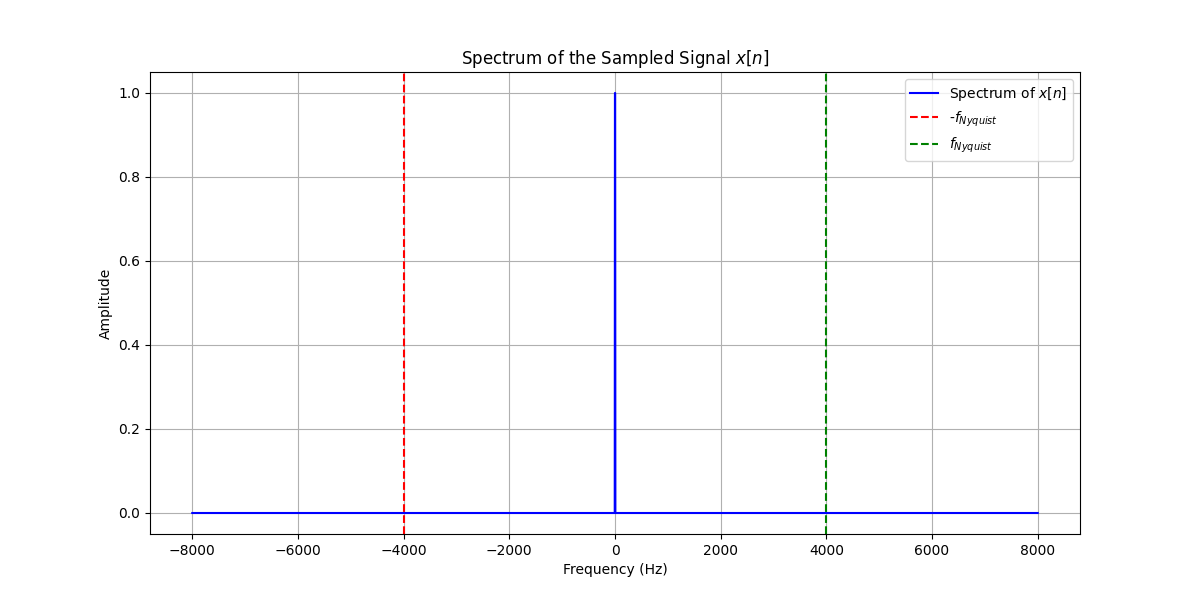
\includegraphics[width=0.8\textwidth]{fig/ex2_task_b_spectrum}
    \caption{Spectrum of \(x[n]\)}
    \label{fig:exercise2b_spectrum}
\end{figure}

\subsection*{Conclusion}
The plotted spectrum effectively illustrates the challenges and considerations needed when designing digital systems that involve sampling.
The clear visibility of the baseband and aliasing effects aids in understanding the importance of maintaining spectrum integrity through appropriate sampling strategies.
